% Relatório técnico do ciclo 3 (INF99003), no modelo enviado pela professora.
% Compilar nesta pasta: pdflatex relatorio_tecnico && pdflatex relatorio_tecnico
\documentclass[11pt,a4paper]{article}

% --- Pacotes Fundamentais ---
\usepackage[utf8]{inputenc}
\usepackage[T1]{fontenc}
\usepackage[brazilian]{babel}
\usepackage{lmodern}
\usepackage[top=2.5cm, bottom=2.5cm, left=2.5cm, right=2.5cm]{geometry}
\usepackage{amsmath,amssymb}
\usepackage{graphicx}
\usepackage{booktabs}
\usepackage{listings}
\usepackage{xcolor}
\usepackage{fancyhdr}
\usepackage[most]{tcolorbox}
\usepackage{hyperref}
% --- Acrescentados pelo grupo (tabelas, gráficos e figuras) ---
\usepackage{multirow}
\usepackage{tabularx}
\usepackage{pgfplots}
\pgfplotsset{compat=1.17}
\usepackage{placeins}
\graphicspath{{../figuras/}}

% --- Configurações de Cores e Links ---
\definecolor{primary}{RGB}{16, 54, 98}      % Azul institucional
\definecolor{secondary}{RGB}{41, 128, 185}  % Azul médio
\definecolor{boxbg}{RGB}{245, 248, 252}     % Fundo para caixas de instrução
\definecolor{boxframe}{RGB}{180, 205, 230}  % Borda das caixas de instrução
\definecolor{codebg}{RGB}{248, 249, 250}

\hypersetup{
    colorlinks=true,
    linkcolor=primary,
    citecolor=secondary,
    urlcolor=secondary
}

% --- Caixa de Instrução para os Alunos ---
\newtcolorbox{instrucao}{
    enhanced,
    colback=boxbg,
    colframe=boxframe,
    arc=3mm,
    boxrule=0.8pt,
    left=4mm, right=4mm, top=3mm, bottom=3mm,
    fonttitle=\bfseries\small\color{primary},
    title={Orientações para esta seção:},
    fontupper=\small\itshape\color{black!80}
}

% --- Configurações para Código-Fonte (Listings) ---
\lstset{
    backgroundcolor=\color{codebg},
    basicstyle=\ttfamily\footnotesize,
    breaklines=true,
    frame=single,
    rulecolor=\color{black!20},
    numbers=left,
    numberstyle=\tiny\color{black!40},
    keywordstyle=\color{primary}\bfseries,
    commentstyle=\color{green!50!black}\itshape,
    stringstyle=\color{orange!80!black},
    extendedchars=true,
    literate={á}{{\'a}}1 {à}{{\`a}}1 {ã}{{\~a}}1 {â}{{\^a}}1 {é}{{\'e}}1 {ê}{{\^e}}1
             {í}{{\'i}}1 {ó}{{\'o}}1 {õ}{{\~o}}1 {ô}{{\^o}}1 {ú}{{\'u}}1 {ç}{{\c{c}}}1
             {Á}{{\'A}}1 {É}{{\'E}}1 {Ó}{{\'O}}1 {Ç}{{\c{C}}}1 {τ}{{$\tau$}}1 {δ}{{$\delta$}}1
             {π}{{$\pi$}}1 {μ}{{$\mu$}}1 {λ}{{$\lambda$}}1 {≤}{{$\le$}}1 {≥}{{$\ge$}}1 {←}{{$\leftarrow$}}1
}
\lstdefinelanguage{pseudo}{
    morekeywords={para,cada,faça,se,então,senão,enquanto,devolva,função,até,pare,e,ou,não},
    sensitive=true,
    morecomment=[l]{//}
}

% --- Cabeçalho e Rodapé ---
\pagestyle{fancy}
\fancyhf{}
\lhead{\footnotesize Projeto em Ciência e Inovação -- 2026/2}
\rhead{\footnotesize Relatório Técnico - Ciclo 3}
\cfoot{\thepage}

% Dados ainda a preencher pelo grupo aparecem em vermelho no PDF.
\newcommand{\preencher}[1]{\textcolor{red}{#1}}
\newcommand{\pp}{\,p.p.}

% ==============================================================================
% DADOS DO TRABALHO
% ==============================================================================
\title{
    \vspace{-1.0cm}
    \textbf{\Large PHVD-APS: planejamento mensal de visitas domiciliares a pé na Atenção Primária à Saúde, com replanejamento após faltas}\\[0.3cm]
    \large Relatório Técnico de Pesquisa e Desenvolvimento (P\&D)
}

\author{
    \textbf{Gabriel P. Knopp} (Cartão: 00594975) -- \texttt{gabriel.knopp@inf.ufrgs.br}\\
    \textbf{Matheus M. Cezar} (Cartão: 00597894) -- \texttt{mmcezar@inf.ufrgs.br}\\
    \textbf{Thiago N. da Fontoura} (Cartão: {00601238}) -- \texttt{tnfontoura@inf.ufrgs.br}\\[0.3cm]
    \normalsize Instituto de Informática -- Universidade Federal do Rio Grande do Sul (UFRGS)\\
    \normalsize Disciplina: Projeto em Ciência e Inovação (2026/2)\\
    \small Primeira versão do artefato (ciclo 2): Fabio Cieslak, Tobias Marion e Vitor Feijo\\
    \small Repositório do Projeto: \url{https://github.com/vitorsfeijo/inf99003-project_2-group_A}
}

\date{Porto Alegre, \today}

% ==============================================================================
% INÍCIO DO DOCUMENTO
% ==============================================================================
\begin{document}

\maketitle
\thispagestyle{fancy}

\begin{abstract}
\noindent
\textbf{Resumo.}
As equipes da Atenção Primária à Saúde montam à mão a agenda de visitas domiciliares: quem visitar, em que dia, com que equipe e em que ordem, a pé, com jornada limitada e prazos clínicos diferentes por paciente. Modelamos o problema como roteamento periódico com seleção de visitas, prazos ponderados pela prioridade clínica e restrições levantadas com agentes de saúde. A hipótese central é que uma busca local sobre o mês inteiro, que realoca e troca visitas entre dias e equipes sob um orçamento de caminhada, atende mais prioridade clínica a tempo do que regras simples, sem caminhar mais. A solução calcula as caminhadas com Dijkstra no OpenStreetMap, melhora cada rota com 1.5-opt e recusa planos inválidos num verificador formal. Comparamos os métodos em pares, com pacientes sintéticos nos territórios do GeoSaúde de Porto Alegre e os mesmos sorteios de faltas. Em 131 territórios, a busca atendeu a tempo 34,63\% dos pontos de prioridade, contra 28,18\% do vizinho mais próximo, com 1,1\% menos caminhada; numa grade de 324 cenários, venceu 899 de 972 pares, mas caminhou 3,03\% mais; com 250 pacientes, concluiu as visitas 5,6 dias úteis antes do vizinho. A hipótese de prioridade foi sustentada nos três estudos, a de deslocamento foi refutada na grade, e nenhum dos 900 planos aleatórios violou as restrições checadas. Os resultados são descritivos e, como o mapa dos estudos não cobre o extremo sul da cidade, os da grade e dos 250 pacientes são provisórios e os dos 131 territórios pedem cautela.
\\[0.3cm]
\textbf{Palavras-chave:} Pesquisa e Desenvolvimento (P\&D); Método Científico; Hipóteses; Avaliação Experimental; Estruturas de Dados; Dados Abertos; Atenção Primária à Saúde; Roteamento de Veículos; Busca Local.
\end{abstract}

\vspace{0.3cm}
\hrule
\vspace{0.4cm}

% ------------------------------------------------------------------------------
\section{Contexto e Definição do Problema}

A Estratégia Saúde da Família organiza equipes multiprofissionais responsáveis pela população de um território definido~\cite{pnab2017,faria2020}. A visita domiciliar é uma de suas ações centrais: alcança quem não consegue ir à unidade, como pessoas acamadas, e sustenta o acompanhamento periódico de condições crônicas~\cite{conass2021}. Na prática, a agenda dessas visitas é montada à mão. A falta de sistemas que acompanhem pendências e intervalos entre visitas é uma fragilidade conhecida da APS~\cite{rodrigues2014}, e o uso de tecnologia da informação nas unidades brasileiras ainda é desigual~\cite{bender2021,pinto2024}.

O problema exige solução computacional porque combina quatro decisões que dependem umas das outras: selecionar as visitas, escolher o dia, atribuir a equipe e ordenar as casas de cada rota a pé. A decisão de hoje muda a carga e os prazos dos dias seguintes, e cada falta de um paciente obriga a refazer o plano. Mesmo um território pequeno, com 30 pacientes e 22 dias úteis, tem combinações demais para conferir de cabeça.

Em 06/11/2026 ouvimos agentes de saúde, e cada pedido virou uma regra do planejador: visitas com data obrigatória, visitas que exigem uma categoria profissional ou mais de uma pessoa (pacientes acamados), pacientes sempre atendidos pela mesma equipe, microáreas cujo contorno não coincide com quem a unidade atende, trechos onde não é seguro passar e folga entre visitas para absorver imprevistos.

\paragraph{Bases de dados.} O projeto usa duas bases abertas e uma sintética:
\begin{itemize}
    \item \textbf{GeoSaúde, Território Base (jul.\ 2025)}~\cite{geosaude}: arquivo KMZ da Prefeitura de Porto Alegre com os polígonos dos territórios das unidades de APS e os pontos das unidades. Usamos os 132 territórios de unidades de saúde.
    \item \textbf{OpenStreetMap}~\cite{haklay2008}: extrato da Região Sul do Brasil distribuído pela Geofabrik~\cite{geofabrik} em formato PBF (cerca de 430~MB, baixado em 08/11/2026). Dele extraímos a rede de caminhada de Porto Alegre: 166.538 nós e 190.780 trechos de via. Essa rede alimenta o roteador interno do aplicativo; as matrizes dos estudos E1 a E3 vieram do OSRM, sobre outro extrato (Seção~5.3).
    \item \textbf{Pacientes sintéticos}: localizações sorteadas dentro dos polígonos e perfis clínicos (condições, intervalos máximos entre visitas, pesos de prioridade de 1 a 5, datas da última visita) gerados com o gerador pseudoaleatório Mulberry32 e sementes fixas. Nenhum dado de paciente real foi usado.
\end{itemize}

\subsection{Formulação do Problema Computacional}

\paragraph{Entradas.} Uma unidade de saúde (nó~0) atende os pacientes $P$ de um território dado por polígonos. Cada paciente $p$ tem localização e condições $C_p$. A condição $c$ tem a última visita $\ell_c$, o intervalo máximo $I_c$, o peso clínico $w_c \in \{1,\dots,5\}$ e o prazo $d_c = \ell_c + I_c$. A janela de planejamento tem $N$ dias úteis (segunda a sexta, sem descontar feriados) $t_1 < \dots < t_N$, com antecipação máxima de $A$ dias corridos. Cada equipe $k \in K$ tem jornada diária de $T_k$ minutos, dias disponíveis e profissionais por categoria. Uma matriz, possivelmente assimétrica, dá o tempo $\tau_{ij}$ e a distância $\delta_{ij}$ a pé entre os nós.

\paragraph{Demanda.} Cada paciente gera no máximo uma visita candidata $v$ na janela, ligada à condição de prazo mais próximo, com prazo $d_v$, peso $w_v$ e tempo de serviço $s_v$ (atendimento mais folga). A visita entra na demanda se já venceu, se vence dentro da antecipação $A$ ou se tem prazo rígido.

\paragraph{Restrições.} Uma solução põe cada candidata em no máximo uma rota $r_{k,t}$ (equipe $k$, dia $t$), ou a deixa pendente com um motivo. Cada rota sai da unidade e volta a ela, e respeita:
\begin{itemize}
    \item \emph{jornada}: $\sum_{(i,j)\in r} \tau_{ij} + \sum_{v\in r} s_v \le T_k$;
    \item \emph{compatibilidade}: a equipe tem as categorias, as quantidades por categoria e o número total de profissionais que a visita exige, e é a equipe vinculada ao paciente, se houver vínculo;
    \item \emph{disponibilidade}: a equipe trabalha no dia $t$, e o paciente não está ausente em $t$;
    \item \emph{prazo rígido}: uma visita com prazo rígido $h_v$ vai para um dia $t \le h_v$; se isso for impossível, fica pendente como obrigatória, com o motivo;
    \item \emph{território}: só entram pacientes dentro dos polígonos, os incluídos explicitamente pela equipe e os não transferidos para outra unidade.
\end{itemize}

\paragraph{Saídas e critérios.} A saída é um plano: para cada dia e equipe, a sequência de visitas com horários previstos, e a lista de pendências com motivo. Seja $t(v)$ o dia atribuído a $v$ (para pendências, $t_N$) e $W = \sum_v w_v$. Os critérios são a prioridade atendida a tempo $\Phi$, o atraso controlável ponderado $\Delta$ e a distância percorrida $D$:
\begin{align}
  \Phi &= \frac{100}{W} \sum_{v \text{ atendida}} w_v \, \bigl[\, t(v) \le \max(d_v, t_1) \,\bigr], \label{eq:phi}\\
  \Delta &= \frac{1}{W}\sum_{v} w_v \, \max\bigl(0,\; t(v) -
\max(d_v, t_1)\bigr), \label{eq:delta}\\
  D &= \textstyle\sum_{r}\sum_{(i,j)\in r} \delta_{ij}. \label{eq:dist}
\end{align}
Em~\eqref{eq:phi} e~\eqref{eq:delta}, uma visita já vencida no início conta como a tempo se feita no primeiro dia, porque o atraso anterior à janela não depende do plano.

\paragraph{Replanejamento.} Ao fim de cada dia, cada visita é registrada como concluída ou não realizada. Só a concluída atualiza $\ell_c$; a não realizada volta à demanda com o prazo original, e o plano é refeito a partir do próximo dia útil.

O problema generaliza o problema de roteamento de veículos com capacidade~\cite{dantzig1959,toth2014} (basta $N=1$ e uma demanda que caiba na jornada) e, portanto, é NP-difícil. Ele combina o roteamento periódico~\cite{campbell2014}, a seleção de visitas dos problemas de orientação~\cite{vansteenwegen2011} e o replanejamento dos problemas dinâmicos~\cite{pillac2013}, num contexto já descrito pelas revisões de atenção domiciliar~\cite{fikar2017,cisse2017}. Por isso, a solução usa heurísticas.

% ------------------------------------------------------------------------------
\section{Formulação das Hipóteses de Solução}

A hipótese do projeto foi escrita no ciclo 2, antes dos experimentos: \emph{uma seleção orientada por urgência e prazos, seguida de inserção de menor custo e melhoria local, reduz o atraso acumulado após replanejamentos sem elevar excessivamente o deslocamento ou o tempo computacional}. No ciclo 3, a heurística principal passou a ser a busca mensal da Seção~\ref{sec:algoritmos}, e desdobramos a hipótese em três afirmações que podem ser refutadas pelos dados já definidos no protocolo experimental.

\subsection{Hipóteses Formuladas}
\begin{itemize}
    \item \textbf{Hipótese Principal ($H_1$):} nas mesmas instâncias, com os mesmos sorteios de faltas, a busca mensal atende a tempo uma fração maior dos pontos de prioridade clínica ($\Phi$) e acumula menos atraso controlável ($\Delta$) do que o vizinho mais próximo e do que a regra de urgência. \\
    \textit{Refutação: média de $\Phi$ menor ou igual à de alguma referência, ou mais derrotas do que vitórias nas comparações pareadas de algum estudo.}
    \item \textbf{Hipótese Comparativa ($H_2$):} a busca mensal não caminha mais do que o vizinho mais próximo, que é a referência construída para economizar caminhada. \\
    \textit{Refutação: distância média ($D$) maior que a do vizinho em algum estudo.}
    \item \textbf{Hipótese de custo ($H_3$):} o cálculo de um plano mensal cabe no uso interativo, abaixo de 1~s, para territórios de até 90 pacientes por equipe. \\
    \textit{Refutação: algum plano mensal com até 90 pacientes calculado em 1~s ou mais.}
\end{itemize}
Os limiares de $H_2$ e $H_3$ tornam mensurável o ``sem elevar excessivamente'' da hipótese original. Eles foram fixados por nós neste ciclo, com os dados do ciclo 2 já disponíveis, e por isso valem como critério declarado, não como pré-registro.

\subsection{Métricas de Sucesso}
\begin{itemize}
    \item \textbf{Prioridade atendida a tempo $\Phi$} (\%), Eq.~\eqref{eq:phi}: a métrica principal de $H_1$.
    \item \textbf{Atraso controlável ponderado $\Delta$} (dias, média ponderada pela prioridade), Eq.~\eqref{eq:delta}, para $H_1$.
    \item \textbf{Distância a pé $D$} (km), Eq.~\eqref{eq:dist}, para $H_2$.
    \item \textbf{Cobertura efetiva} (\%): visitas concluídas sobre a demanda inicial inteira.
    \item \textbf{Dias úteis até concluir} um acúmulo de visitas (estudo de 250 pacientes).
    \item \textbf{Tempo de planejamento} (ms), para $H_3$.
    \item \textbf{Violações de restrição}: número de planos recusados pelo verificador formal. A meta é zero, para qualquer estratégia.
\end{itemize}

% ------------------------------------------------------------------------------
\section{Desenvolvimento e Implementação da Solução}

\subsection{Modelagem Computacional e Arquitetura}

O artefato é um monorepo em TypeScript (Node.js 22 ou superior) com três pacotes:
\begin{itemize}
    \item \texttt{@routing/core}: núcleo de planejamento, puro, sem estado e sem dependências externas. Recebe um cenário serializável e devolve um plano verificado.
    \item \texttt{@routing/server}: servidor Fastify com SQLite (WAL e chaves estrangeiras ativas). Versiona cenários, planos e resultados de visitas, calcula as matrizes de caminhada e exporta rotas em CSV, GPX e Excel.
    \item \texttt{@routing/web}: interface em React e Leaflet, com o mapa, as rotas por equipe e dia, o registro do dia e as estatísticas de uso (Fig.~\ref{fig:interface}).
\end{itemize}
As estratégias de planejamento seguem o padrão \emph{Strategy}: só a etapa de distribuição das visitas muda entre os métodos comparados, e todos recebem a mesma demanda e a mesma matriz.

\begin{figure}[ht]
\centering
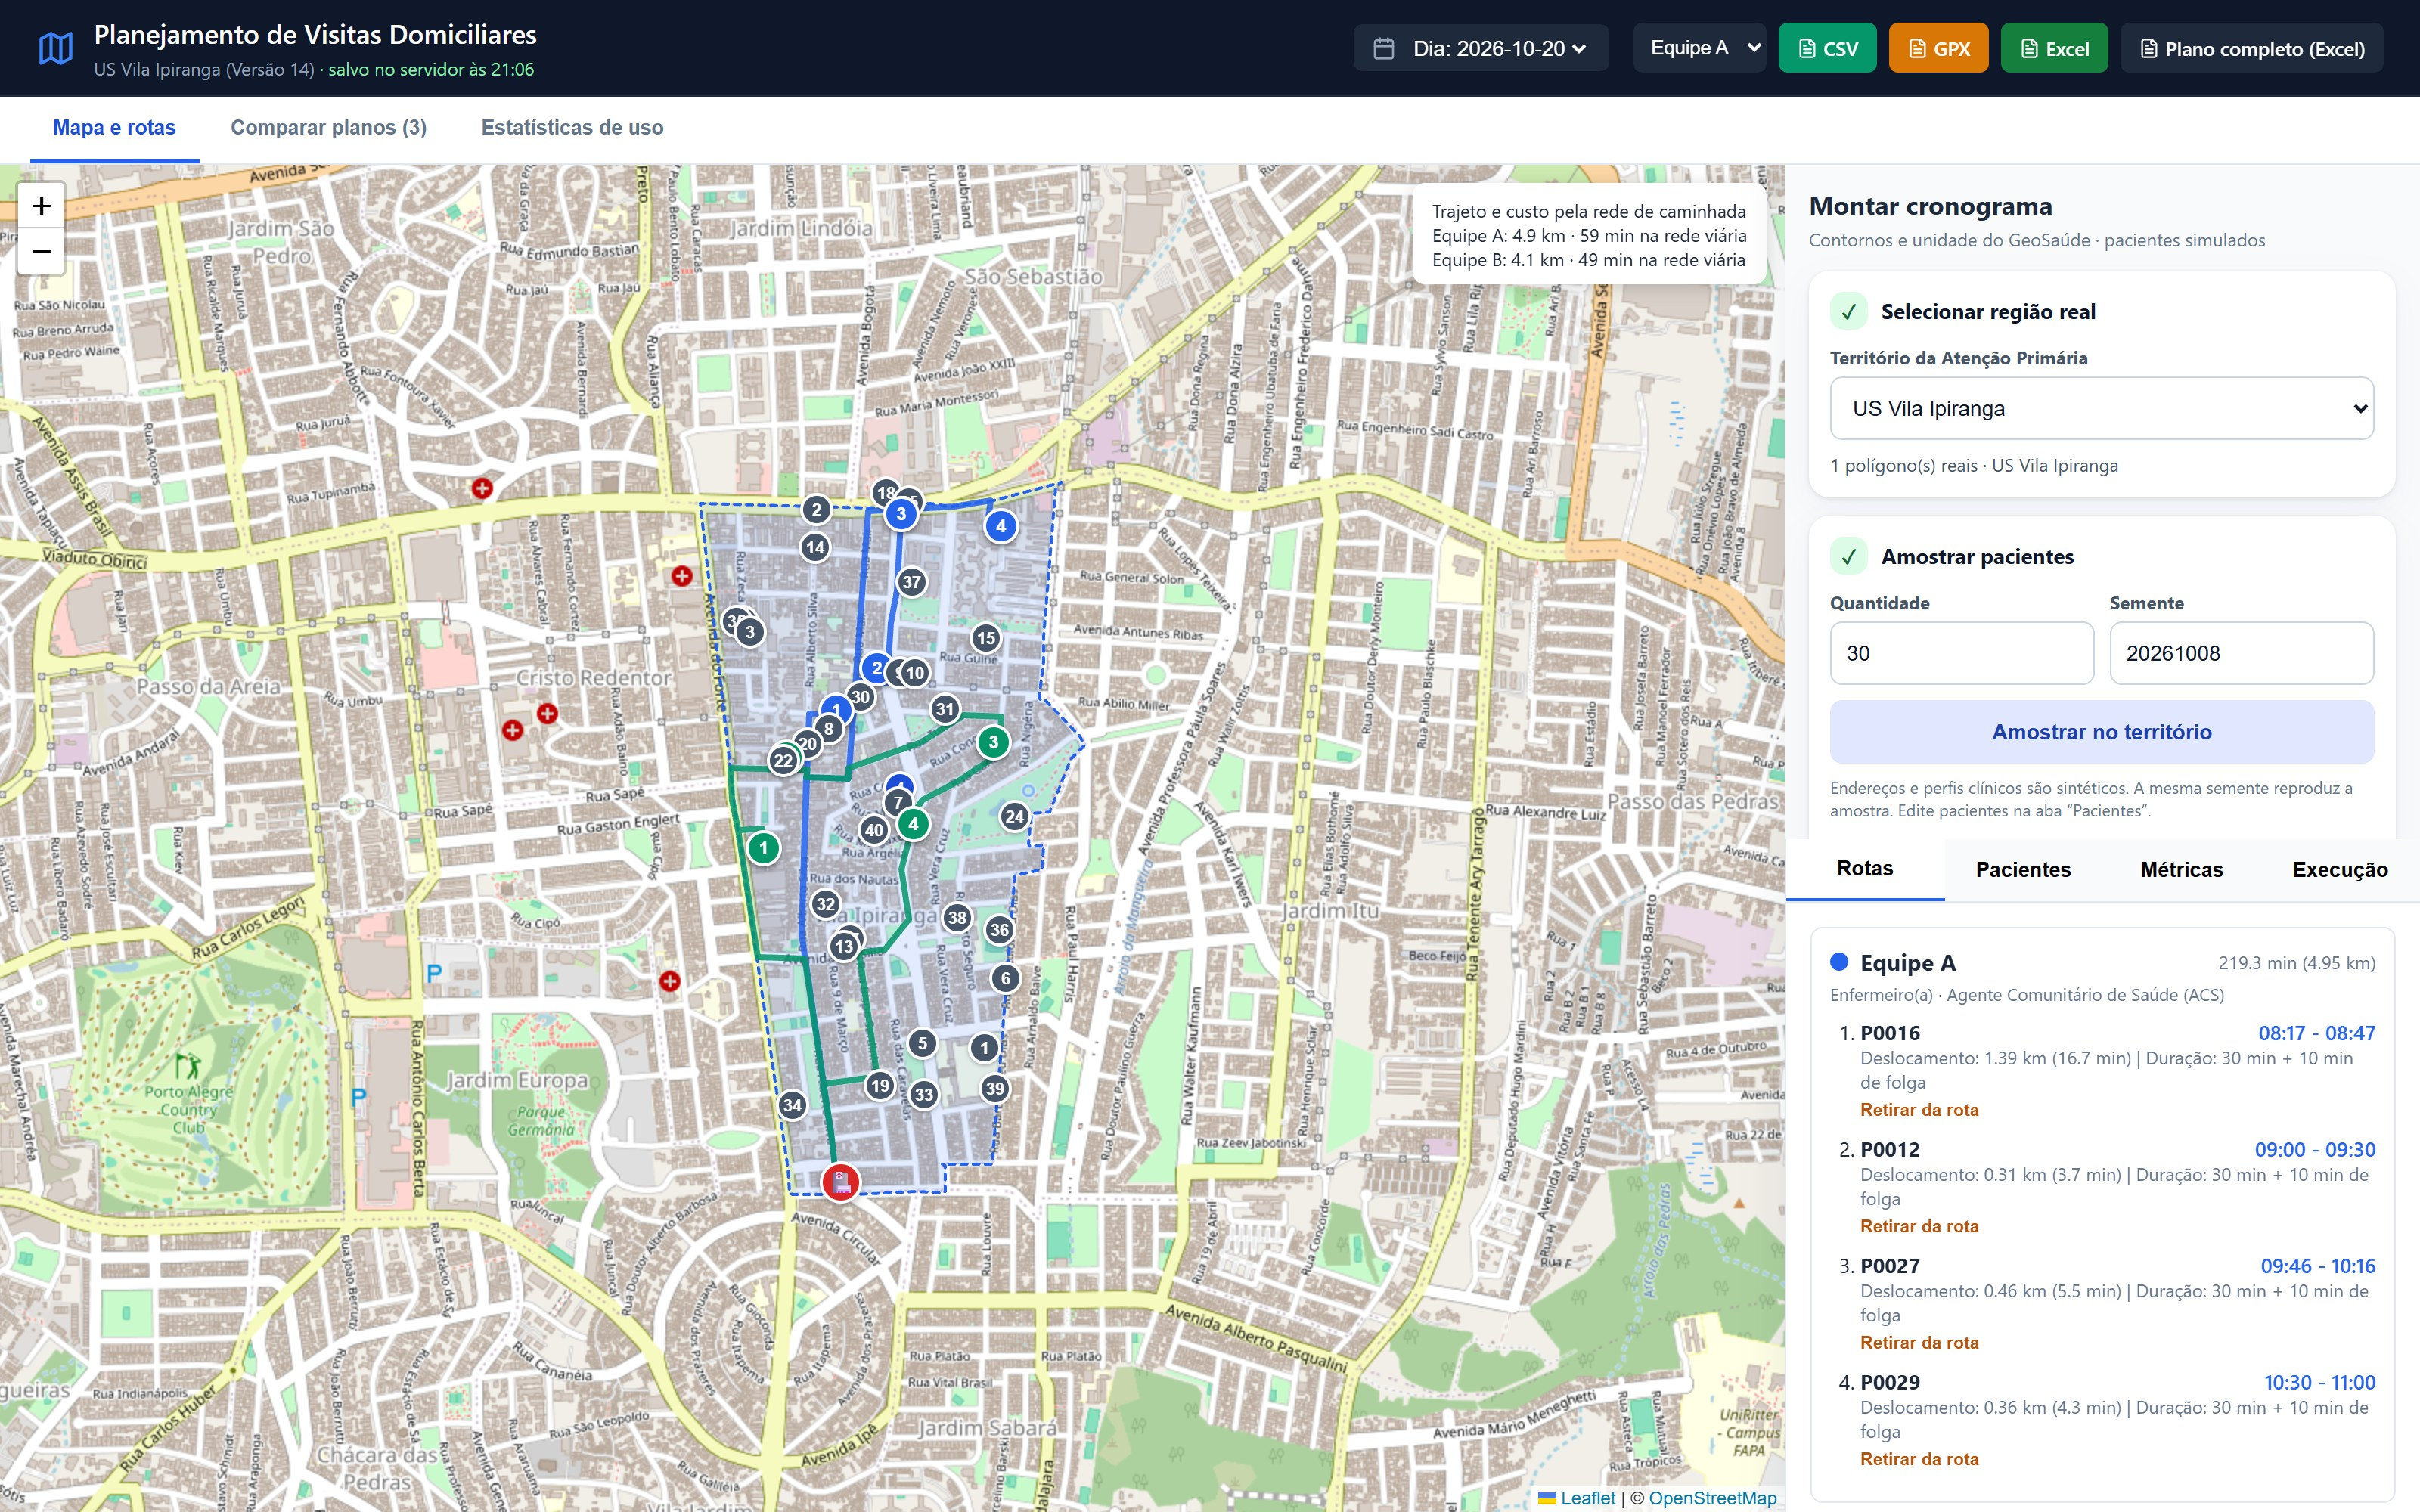
\includegraphics[width=0.92\textwidth]{mapa-rotas.jpg}
\caption{Interface do artefato na US Vila Ipiranga: território do GeoSaúde, pacientes numerados, as rotas a pé das equipes A e B num dia e a agenda do dia na lateral. Pacientes sintéticos.}
\label{fig:interface}
\end{figure}

As entidades do domínio foram mapeadas nestas estruturas de dados:
\begin{itemize}
    \item \textbf{Grafo de caminhada.} Os vértices $V$ são pontos da rede de vias do OpenStreetMap (cruzamentos e pontos de forma), e as arestas $E$ são trechos de via percorríveis a pé, sem sentido único. O grafo usa lista de adjacência compacta (formato CSR): coordenadas em \texttt{Float64Array}, vetor de deslocamentos \texttt{offsets} e destinos \texttt{targets} em \texttt{Uint32Array}, comprimento (m) e duração (s) de cada aresta em \texttt{Float32Array} e o componente conexo de cada nó em \texttt{Uint16Array}. Cada aresta aparece nos dois sentidos: $|V| = 166.538$, $|E| = 190.780$ e 381.560 entradas de adjacência, num arquivo binário de 8~MB carregado sem conversão.
    \item \textbf{Índice espacial em grade.} Para projetar um paciente na via mais próxima, os segmentos de via são indexados numa grade uniforme de células de 100~m, também em formato CSR (início de cada célula e lista de segmentos). A busca examina só as células vizinhas do ponto.
    \item \textbf{Fila de prioridade.} O Dijkstra usa um heap binário mínimo sobre arrays tipados, com carimbos de geração para reaproveitar os vetores de distância entre execuções sem reinicializá-los.
    \item \textbf{Matriz de custos.} Tempo e distância a pé entre a unidade (índice 0) e os pacientes elegíveis, em matrizes densas $(n+1)\times(n+1)$.
    \item \textbf{Tabelas hash.} Mapas de identificador para índice da matriz, para candidata, para equipe e para prioridade dão acesso $O(1)$ durante a busca.
    \item \textbf{Rotas.} Cada rota é uma lista ordenada de visitas indexada por (equipe, dia), com tempo, distância e horários recalculados a partir da matriz.
    \item \textbf{Persistência.} Tabelas SQLite de cenários (com versões), planos e resultados de visitas, e o histórico de alterações do qual saem as estatísticas de uso.
    \item \textbf{Conjuntos disjuntos.} Na construção do grafo, uma estrutura \emph{union-find} identifica os componentes conexos e descarta fragmentos com menos de 500 nós.
\end{itemize}

\subsection{Algoritmos e Análise de Custo/Complexidade}\label{sec:algoritmos}

Todo plano percorre o mesmo pipeline: (1)~validação do cenário e seleção dos pacientes elegíveis; (2)~demanda; (3)~matriz de caminhada, com validação; (4)~estratégia; (5)~garantia de prazos rígidos; (6)~melhoria intra-rota 1.5-opt; (7)~verificação formal. Só a etapa 4 muda entre os métodos, mas a busca mensal também chama internamente a garantia de prazos rígidos e o 1.5-opt (Listagem~\ref{lst:busca}).

\paragraph{Matriz de caminhada.} Cada ponto é projetado no segmento de via mais próximo (erro explícito se estiver a mais de 1~km de qualquer via). A matriz sai de um Dijkstra~\cite{dijkstra1959} a partir de cada origem, interrompido quando todos os destinos foram fixados. O peso de busca é a duração da aresta, a 5~km/h (2,5~km/h em escadas), seguindo o perfil \texttt{foot} do OSRM~\cite{luxen2011}. Ruas que tocam uma área de risco desenhada pela equipe têm o peso multiplicado por 25, mas o tempo e a distância devolvidos são os reais.

\paragraph{Estratégias de referência.} A regra de \emph{urgência} ordena, para cada dia e equipe, as candidatas vencidas ou que vencem no dia por uma pontuação (dias de atraso $\times 10$ + peso $\times 5$) e as acrescenta ao fim da rota enquanto a jornada comportar. O \emph{vizinho mais próximo} parte da unidade e, a cada passo, acrescenta a candidata elegível e viável de menor tempo de caminhada a partir da posição atual (a unidade na primeira escolha e, depois, a última visita da rota), até não haver outra que caiba na jornada.

\paragraph{Busca mensal (heurística principal).} Parte do plano do vizinho mais próximo, garante os prazos rígidos e aplica duas fases de busca local sobre o mês inteiro (Listagem~\ref{lst:busca}). Cada movimento realoca uma visita para outra rota (outro dia ou outra equipe) ou troca duas visitas entre rotas. O ganho de um movimento é
\begin{equation}
  g = \Delta\tau + \lambda \sum w_v\,\Delta a_v - \mu \sum w_v\,\Delta \pi_v,
\end{equation}
em que $\Delta\tau$ é a variação do tempo de caminhada, $a_v$ é o atraso controlável da visita e $\pi_v \in\{0,1\}$ indica atendimento sem atraso. Os pesos $\lambda = 12$ e $\mu = 24$ dizem quantos minutos de caminhada valem um ponto de prioridade atrasado um dia e um ponto atendido prontamente. Eles foram fixados por julgamento, não ajustados aos dados. Um movimento só é aceito se o tempo e a distância totais não superarem os do início da fase (medidos depois da primeira inserção de pendências, quando há recuperação) e se os pontos atendidos prontamente não diminuírem. O orçamento é relativo ao estado inicial de cada fase, não ao plano do vizinho mais próximo: a recuperação de pendências pode aumentar a caminhada antes de o orçamento ser fixado e, ao final, depois dos movimentos.

\begin{lstlisting}[language=pseudo, caption={Busca mensal (simplificada do código em \texttt{main-heuristic.ts}).}, label={lst:busca}, mathescape=true]
função BuscaMensal(candidatas V, dias t1..tN, equipes K, matriz (τ, δ))
  S ← VizinhoMaisPróximo(V)
  S ← GarantirPrazosRígidos(S)      // retira visitas de menor peso se preciso
  S ← Fase(S, recuperar = falso, μ = 0)
  devolva Fase(S, recuperar = verdadeiro, μ = 24)

função Fase(S, recuperar, μ)
  aplicar 1.5-opt a cada rota de S
  se recuperar então inserir pendências pela menor variação de custo
  Bτ, Bδ, Bπ ← tempo, distância e pontos prontos de S   // orçamento da fase
  para até 80 iterações faça
    m ← realocação ou troca viável de menor ganho g,
        com τ(S') ≤ Bτ, δ(S') ≤ Bδ e π(S') ≥ Bπ
    se não há m com g < 0 então pare
    aplicar m; 1.5-opt nas duas rotas alteradas
  se recuperar então
    trocar visitas de peso menor por pendências de peso maior
    (nunca uma visita de prazo rígido) e inserir as que passaram a caber
  devolva S
\end{lstlisting}

\paragraph{Prazos rígidos, 1.5-opt e verificação.} A garantia de prazos rígidos roda depois de qualquer estratégia: percorre as visitas obrigatórias por prazo e as insere na melhor posição viável até o prazo, retirando visitas sem prazo rígido, das de menor peso para as de maior. O 1.5-opt combina reinserção de um nó e inversão de subsegmento (2-opt~\cite{croes1958}) em primeira melhoria, até não haver ganho no tempo da rota. O verificador formal recusa equipe inexistente, indisponível ou incompatível, jornada excedida, paciente repetido, visita em dia de ausência, visita depois do prazo rígido e paciente fora do território. Nenhum plano é devolvido sem passar por ele.

\paragraph{Complexidade.} Sejam $n$ o número de candidatas, $R = |K| \cdot N$ o número de rotas, $L$ o máximo de visitas numa rota (limitado pela jornada) e $n_a \le \min(n, RL)$ o número de visitas alocadas. A Tabela~\ref{tab:complexidade} resume o custo de cada etapa. A avaliação de cada posição recalcula a rota em $O(L)$, o que deixa as fórmulas simples em troca de um fator $L$.

\begin{table}[ht]
\centering
\caption{Custo assintótico das etapas do pipeline}
\label{tab:complexidade}
\small
\begin{tabularx}{\textwidth}{@{}lXl@{}}
\toprule
\textbf{Etapa} & \textbf{Justificativa} & \textbf{Custo} \\
\midrule
Construção do grafo & leitura do PBF, ordenação dos nós e \emph{union-find} & $O(M \log M)$, $M$ = nós do extrato \\
Projeção dos pontos & grade de 100~m: só as células vizinhas & $O(n)$ esperado \\
Matriz de caminhada & um Dijkstra com heap binário por origem~\cite{cormen} & $O\bigl(n\,(|V|+|E|)\log |V|\bigr)$ \\
Demanda & uma passada pelas condições de cada paciente & $O(\sum_p |C_p|)$ \\
Urgência & ordenação e varredura por rota & $O(R\, n \log n)$ \\
Vizinho mais próximo & cada inserção varre as candidatas & $O(R\, L\, n)$ \\
1.5-opt (uma varredura) & $O(L^2)$ movimentos, cada um avaliado
em $O(L)$; repete até não haver ganho & $O(L^3)$ por varredura \\
Busca mensal (uma iteração) & cada visita alocada $\times$ cada rota
$\times$ cada posição, avaliada em $O(L)$; as trocas custam
$O(n_a^2 L) \le O(n_a R L^2)$, pois $n_a \le RL$
& $O(n_a R L^2)$ \\
Recuperação de pendências & só na segunda fase, antes e depois
dos movimentos (três passadas): cada pendência $\times$ cada rota
$\times$ cada posição, avaliada em $O(L)$ & $O\bigl((n-n_a)\, R\, L^2\bigr)$ \\
Busca mensal (total) & até 80 movimentos aceitos por fase, duas
fases, a recuperação de pendências, o 1.5-opt inicial em todas as
rotas e nas rotas alteradas após cada movimento & $O\bigl((160\,
n_a + n)\, R\, L^2\bigr)$ mais o custo do 1.5-opt \\
Verificador formal & uma passada pelas rotas com tabelas hash & $O(R\,L + n)$ \\
\bottomrule
\end{tabularx}
\end{table}

Se $L$ fosse constante, a iteração da busca cresceria como $n_a \cdot R$; na grade, porém, o comprimento médio das rotas cresce com $n_a$ ($L \approx n_a/R$), de modo que a iteração se aproxima de $O(n_a^3/R)$. O limite de 80 iterações garante término, mas, abaixo dele, o número de iterações efetivas também cresce com a instância. Na matriz, a interrupção antecipada do Dijkstra e o tamanho dos territórios (poucos km\textsuperscript{2}) deixam o custo real muito abaixo do limite.

\subsection{Tratamento e Pré-processamento dos Dados}

\paragraph{Territórios.} O KMZ do GeoSaúde é convertido em GeoJSON. Mantemos os polígonos e multipolígonos dos territórios de APS e associamos cada território ao ponto da unidade de mesmo nome, ou ao ponto mais próximo quando o nome não coincide. Cada cenário gerado guarda um registro de proveniência com o arquivo de origem, o hash SHA-256, a forma de associação da unidade, a semente e o método de amostragem.

\paragraph{Rede de caminhada.} Do extrato PBF, mantemos as vias percorríveis a pé com os filtros do perfil \texttt{foot} do OSRM. Aplicamos 5~km/h, 2,5~km/h em escadas e velocidade reduzida em superfícies lentas (cascalho e areia), recortamos o retângulo de Porto Alegre (latitude $-30{,}30$ a $-29{,}92$, longitude $-51{,}32$ a $-50{,}95$) e descartamos componentes conexos com menos de 500 nós (calçadas isoladas e trechos cortados pelo recorte). O grafo é gravado em binário e regerado em cerca de 15~s por \texttt{npm run prepare-map}. Os nós de barreira, as balsas e as restrições de conversão são ignorados.

\paragraph{Pacientes.} Na amostra sintética, as localizações são sorteadas uniformemente dentro dos polígonos (rejeitando pontos fora deles ou em buracos), e os perfis clínicos são copiados de modelos. Quando a unidade usa o próprio cadastro, a importação aceita Excel (.xlsx), CSV (inclusive em Windows-1252, como o Excel em português salva) e JSON. Cada linha com problema (data inexistente, coordenadas trocadas, categoria ou equipe desconhecida) é recusada com o motivo, nunca corrigida em silêncio.

\paragraph{Validação do cenário.} Antes de planejar, \texttt{validateScenario} recusa cenários sem unidade com localização válida, sem polígono de território válido, com janela $N < 1$ ou antecipação negativa, e pacientes ou equipes com valores inválidos (vínculo a equipe inexistente, quantidades de profissionais, durações ou períodos de ausência inválidos). Os pacientes fora do território e os transferidos são excluídos do planejamento, com aviso, e não entram no denominador das métricas. O núcleo também confere os identificadores, as dimensões e os valores da matriz (finitos e não negativos) antes de planejar.

% ------------------------------------------------------------------------------
\section{Projeto Experimental e Metodologia de Validação}

\subsection{Ambiente Experimental e Variáveis}
\begin{itemize}
    \item \textbf{Ambiente:} TypeScript 5.4 executado em Node.js; matrizes de E1 a E3 obtidas da API Table do OSRM com o perfil \texttt{foot}, sobre o extrato \texttt{PortoAlegre.osm.pbf} da BBBike (ver ``Mapa dos estudos'' na Seção~5.3), guardadas em cache e reaproveitadas em toda reexecução. A grade fatorial foi reexecutada em 22/11/2026 num AMD Ryzen 7 5700X3D (8 núcleos), 32~GB de RAM, Windows 11 Pro e Node.js 26.13, e as Tabelas~\ref{tab:fatorial} e~\ref{tab:experimentos} vêm dessa execução. Os tempos de E1 e E3 vêm da execução original, cuja máquina não foi registrada nos arquivos de resultado.
    \item \textbf{Variáveis Independentes:} estratégia (busca mensal, vizinho mais próximo, urgência); território; número de pacientes $n$; área do território; horizonte $N$; proporção de visitas já vencidas no início; probabilidade de falta por tentativa.
    \item \textbf{Variáveis Dependentes:} $\Phi$, $\Delta$, $D$, cobertura efetiva, dias úteis até concluir um acúmulo, tempo de planejamento e número de planos recusados pelo verificador.
    \item \textbf{Variáveis de Controle:} em cada comparação, as três estratégias recebem a mesma demanda, a mesma matriz, a mesma equipe (240~min/dia, 300~min/dia em E3), $A = 2$ dias e os mesmos sorteios de falta (números aleatórios comuns por paciente e data); sementes fixas; uma execução por configuração, sem descarte de aquecimento nem repetição, porque as métricas de plano são determinísticas; por isso os tempos incluem o efeito da compilação JIT nas primeiras execuções, e o desvio-padrão da Tabela~\ref{tab:experimentos} reflete a variação entre cenários, não o ruído de medição.
\end{itemize}

\subsection{Cenários e Protocolo de Coleta}

A simulação executa cada dia útil: sorteia a falta de cada visita planejada, registra concluída ou não realizada e refaz o plano a partir do próximo dia útil. Instâncias sem caminho a pé completo entre todos os pontos são excluídas e listadas em \texttt{exclusions.json}. Quatro estudos foram executados:
\begin{itemize}
    \item \textbf{E1, cidade inteira} ($H_1$, $H_2$): 131 territórios do GeoSaúde com caminho completo (1 dos 132 excluído), 30 pacientes cada, uma equipe, 22 dias úteis e faltas de 0\%, 5\% e 10\%: $131 \times 3 = 393$ comparações pareadas por referência.
    \item \textbf{E2, grade fatorial} ($H_1$, $H_2$, $H_3$): território da US Restinga; 3 sementes $\times$ 4 quantidades de pacientes (15, 30, 45 e 90) $\times$ 3 áreas (0,5, 1 e 2 vezes o polígono) $\times$ 3 horizontes (5, 10 e 22 dias úteis) $\times$ 3 proporções de visitas já vencidas (0, 25\% e 50\%) $= 324$ cenários; $\times$ 3 níveis de falta $= 972$ pares por referência.
    \item \textbf{E3, acúmulo de 250 pacientes} ($H_1$, $H_2$): Restinga, prazos entre outubro de 2026 e janeiro de 2027, limite comum de 12 meses (261 dias úteis); 3 sementes $\times$ 3 níveis de falta $= 9$ pares; mede os dias úteis até concluir as 250 visitas.
    \item \textbf{E4, propriedades}: 300 cenários sorteados com restrições combinadas (datas obrigatórias, categorias e quantidades, vínculos, ausências, folgas, equipes de folga), nas três estratégias, totalizando 900 planos.
\end{itemize}

\paragraph{Consolidação estatística.} As comparações são pareadas: no mesmo cenário e com o mesmo nível de falta, comparamos a busca mensal a cada referência e contamos vitórias, empates e derrotas. Relatamos médias, medianas e, para o tempo, o máximo. Não aplicamos testes de hipótese nem intervalos de confiança: os pares de um mesmo cenário compartilham pacientes e sorteios entre os níveis de falta e não são independentes, e as sementes são poucas. Os números são descritivos~\cite{wohlin2012}.

\paragraph{Testes automáticos.} Além dos estudos, o núcleo tem 47 testes (métricas, busca mensal, amostragem, restrições, limites, operações de campo e importação) e o servidor tem 3 (leitura de planilhas .xlsx).

% ------------------------------------------------------------------------------
\section{Resultados Experimentais e Discussão}

\subsection{Apresentação dos Dados Coletados}

\paragraph{E1, cidade inteira.} A Tabela~\ref{tab:cidade} resume as 393 execuções pareadas de cada estratégia. A busca mensal atendeu a tempo 34,63\% dos pontos de prioridade, 6,45\pp\ acima do vizinho mais próximo, e caminhou 1,1\% menos. Venceu 307 dos 393 pares em $\Phi$, empatou 58 e perdeu 28. A cobertura quase não muda entre os métodos (a da busca mensal é a menor das três: 98,07\% contra 98,23\% e 98,55\%): o ganho está em \emph{quando} e \emph{quem} é atendido, não em quantos.

\begin{table}[ht]
\centering
\caption{E1: médias em 131 territórios $\times$ 3 níveis de falta (simulação de 22 dias úteis); tempos da execução original, em máquina não registrada; mapa BBBike incompleto ao sul (Seção~5.3)}
\label{tab:cidade}
\begin{tabular}{@{}lrrr@{}}
\toprule
\textbf{Indicador} & \textbf{Busca mensal} & \textbf{Vizinho} & \textbf{Urgência} \\
\midrule
Prioridade a tempo $\Phi$ (\%) & \textbf{34,63} & 28,18 & 17,93 \\
Cobertura efetiva (\%) & 98,07 & 98,23 & 98,55 \\
Atraso controlável $\Delta$ (dias) & \textbf{2,76} & 3,07 & 3,69 \\
Distância a pé $D$ (km) & \textbf{69,60} & 70,40 & 97,06 \\
Tempo de planejamento acumulado (ms) & 131,87 & 12,78 & 9,00 \\
\bottomrule
\end{tabular}
\end{table}

\paragraph{E2, grade fatorial.} A Tabela~\ref{tab:fatorial} traz o ganho pareado da busca mensal. Frente ao vizinho, ganhou em média 9,65\pp\ de $\Phi$ e 0,55 dia de atraso, mas caminhou 3,03\% mais (113,16 contra 109,83~km) e caminhou mais em 473 dos 972 pares. Frente à urgência, venceu todos os 972 pares em $\Phi$ e em atraso. O ganho frente ao vizinho cai pouco com a taxa de faltas (Fig.~\ref{fig:faltas}). Este estudo usou o extrato de mapa que não cobria a Restinga (Seção~5.3): os quilômetros absolutos, e possivelmente a comparação de distância, não são representativos.

\begin{table}[ht]
\centering
\caption{E2: ganho pareado da busca mensal sobre cada referência (972 pares)}
\label{tab:fatorial}
\begin{tabular}{@{}llrrr@{}}
\toprule
\textbf{Referência} & \textbf{Métrica} & \textbf{Média} & \textbf{Mediana} & \textbf{V/E/D} \\
\midrule
\multirow{4}{*}{Vizinho} & Prioridade a tempo (p.p.) & 9,65 & 6,62 & 899/64/9 \\
 & Atraso controlável (dias) & 0,55 & 0,39 & 943/6/23 \\
 & Distância (km) & $-$3,33 & 0,00 & 284/215/473 \\
 & Cobertura (p.p.) & 0,90 & 0,00 & 271/619/82 \\
\midrule
\multirow{4}{*}{Urgência} & Prioridade a tempo (p.p.) & 20,84 & 18,37 & 972/0/0 \\
 & Atraso controlável (dias) & 2,07 & 1,46 & 972/0/0 \\
 & Distância (km) & 21,54 & 15,30 & 813/77/82 \\
 & Cobertura (p.p.) & 12,50 & 12,78 & 635/324/13 \\
\bottomrule
\multicolumn{5}{@{}p{0.92\textwidth}@{}}{\footnotesize Ganho positivo favorece a busca mensal; em distância, negativo significa mais caminhada. V/E/D: vitórias, empates e derrotas.}
\end{tabular}
\end{table}

\begin{figure}[ht]
\centering
\begin{tikzpicture}
\begin{axis}[
  width=0.7\textwidth, height=5cm,
  ybar, bar width=12pt, ymin=0, ymax=12,
  symbolic x coords={0\%,5\%,10\%}, xtick=data,
  xlabel={Probabilidade de falta por tentativa}, ylabel={Ganho em $\Phi$ (p.p.)},
  legend style={at={(0.5,1.03)}, anchor=south, legend columns=2, draw=none},
  nodes near coords, nodes near coords style={font=\scriptsize, /pgf/number format/use comma, /pgf/number format/fixed, /pgf/number format/precision=2},
  enlarge x limits=0.25]
\addplot[fill=black!25, draw=black!60] coordinates {(0\%,6.91) (5\%,6.52) (10\%,5.94)};
\addplot[fill=secondary!60, draw=primary] coordinates {(0\%,9.91) (5\%,9.57) (10\%,9.47)};
\legend{E1 (cidade), E2 (fatorial)}
\end{axis}
\end{tikzpicture}
\caption{Ganho médio de prioridade atendida a tempo da busca mensal sobre o vizinho mais próximo, por taxa de faltas.}
\label{fig:faltas}
\end{figure}

\paragraph{E3, acúmulo de 250 pacientes.} Nos 9 pares, a busca mensal concluiu as 250 visitas em 88,11 dias úteis, contra 93,67 do vizinho ($-5{,}56$) e 89,78 da urgência ($-1{,}67$), e caminhou 13,03\% menos que o vizinho (Tabela~\ref{tab:longo}). Frente ao vizinho, a vantagem em dias cresce com as faltas, de 3,67 para 8,33 dias úteis; frente à urgência ela é pequena (0,66 a 3,34 dias úteis) e, com 3 sementes, diferenças menores que um dia não são distinguíveis. Na prioridade, a busca atendeu a tempo 49,05\% dos pontos, contra 30,22\% do vizinho e 16,05\% da urgência, com atraso controlável $\Delta$ de 5,13 dias, contra 11,49 e 12,33, e venceu os 9 pares nas duas métricas frente a cada referência. Todas as 27 execuções concluíram as 250 visitas. Este estudo usou o extrato de mapa que não cobria a Restinga (Seção~5.3): os valores absolutos de dias e quilômetros não são representativos.

\begin{table}[ht]
\centering
\caption{E3: dias úteis até concluir 250 visitas e caminhada total (médias de 3 sementes)}
\label{tab:longo}
\begin{tabular}{@{}lrrrrrr@{}}
\toprule
& \multicolumn{2}{c}{\textbf{Busca mensal}} & \multicolumn{2}{c}{\textbf{Vizinho}} & \multicolumn{2}{c}{\textbf{Urgência}} \\
\cmidrule(lr){2-3}\cmidrule(lr){4-5}\cmidrule(l){6-7}
\textbf{Faltas} & dias & km & dias & km & dias & km \\
\midrule
0\% & \textbf{87,67} & \textbf{1.103} & 91,33 & 1.273 & 88,33 & 1.342 \\
5\% & \textbf{88,33} & \textbf{1.123} & 93,00 & 1.291 & 89,33 & 1.419 \\
10\% & \textbf{88,33} & \textbf{1.179} & 96,67 & 1.352 & 91,67 & 1.460 \\
\bottomrule
\end{tabular}
\end{table}

\paragraph{Tempo de planejamento em função de $n$.} A Tabela~\ref{tab:experimentos} e a Fig.~\ref{fig:tempo} mostram o tempo de cálculo do plano inicial na grade fatorial, por número de pacientes. Cada linha reúne 81 cenários (3 sementes $\times$ 3 áreas $\times$ 3 horizontes $\times$ 3 proporções de vencidas).

\begin{table}[ht]
\centering
\caption{Desempenho comparativo de tempo em função do tamanho da entrada $n$ (plano inicial, grade fatorial, 81 cenários por linha)}
\label{tab:experimentos}
\resizebox{\textwidth}{!}{%
\begin{tabular}{@{}cccccc@{}}
\toprule
\textbf{Entrada ($n$)} & \textbf{Busca mensal} & \textbf{Busca mensal} & \textbf{Vizinho} & \textbf{Urgência} & \textbf{Visitas alocadas} \\
\textbf{pacientes} & \textbf{média $\pm$ dp (ms)} & \textbf{mediana / máx.\ (ms)} & \textbf{média $\pm$ dp (ms)} & \textbf{média $\pm$ dp (ms)} & \textbf{(busca, média)} \\ \midrule
15 & 6,47 $\pm$ 4,59 & 5,38 / 21,6 & 0,40 $\pm$ 0,07 & 0,31 $\pm$ 0,09 & 13,4 \\
30 & 21,39 $\pm$ 17,93 & 14,67 / 83,2 & 0,96 $\pm$ 0,17 & 0,58 $\pm$ 0,14 & 24,2 \\
45 & 42,35 $\pm$ 40,02 & 25,64 / 170,6 & 1,72 $\pm$ 0,30 & 0,90 $\pm$ 0,21 & 31,1 \\
90 & 118,28 $\pm$ 131,11 & 70,29 / 570,9 & 4,86 $\pm$ 1,19 & 1,98 $\pm$ 0,57 & 45,9 \\ \bottomrule
\end{tabular}%
}
\end{table}

\begin{figure}[ht]
\centering
\begin{tikzpicture}
\begin{loglogaxis}[
  width=0.7\textwidth, height=5.5cm,
  xlabel={Pacientes ($n$)}, ylabel={Tempo médio (ms)},
  xtick={15,30,45,90}, xticklabels={15,30,45,90},
  legend style={at={(0.5,-0.32)}, anchor=north, legend columns=3, font=\footnotesize, draw=none},
  grid=major, grid style={black!10}]
\addplot[mark=*, color=primary, thick] coordinates {(15,6.47) (30,21.39) (45,42.35) (90,118.28)};
\addplot[mark=square*, color=secondary] coordinates {(15,0.40) (30,0.96) (45,1.72) (90,4.86)};
\addplot[mark=triangle*, color=black!50] coordinates {(15,0.31) (30,0.58) (45,0.90) (90,1.98)};
\legend{Busca mensal ($\approx n^{1{,}62}$), Vizinho ($\approx n^{1{,}40}$), Urgência ($\approx n^{1{,}04}$)}
\end{loglogaxis}
\end{tikzpicture}
\caption{Tempo médio de planejamento em escala log-log. O expoente entre parênteses é a inclinação entre $n=15$ e $n=90$.}
\label{fig:tempo}
\end{figure}

Com o horizonte, o tempo da busca mensal passa de 10,99~ms (5 dias) para 34,31~ms (10 dias) e 96,07~ms (22 dias); o do vizinho, de 1,59 para 2,42~ms. Nas simulações dinâmicas, cada replanejamento da busca levou 16,1~ms em média e 160,6~ms no pior caso.

\paragraph{E4, propriedades.} Os 900 planos foram aceitos pelo verificador, sem visitas duplicadas, com equipes compatíveis, horários ordenados, totais de rota iguais aos da matriz e jornadas respeitadas. Toda visita de prazo rígido foi agendada a tempo ou ficou pendente como obrigatória, com o motivo. Isso mostra ausência de violações nos 900 planos sorteados, não que o sistema nunca viole uma restrição. Para estimar a sensibilidade dos testes, desativamos no código compilado, uma de cada vez, a regra de ausência e a de quantidade por categoria: as suítes falharam nos dois casos. As outras regras não foram testadas dessa forma.

\subsection{Validação ou Refutação das Hipóteses}
\begin{itemize}
    \item \textbf{Hipótese $H_1$ (prioridade e atraso): sustentada nos três estudos, de modo provisório em E2 e E3.} Nos três estudos, a busca mensal teve $\Phi$ médio maior e $\Delta$ menor que as duas referências, e mais vitórias do que derrotas em $\Phi$: frente ao vizinho, 307/58/28 em E1, 899/64/9 em E2 e 9/0/0 em E3; frente à urgência, 972/0/0 em E2 e 9/0/0 em E3. Em E3, a busca também concluiu as 250 visitas 5,56 dias úteis antes do vizinho e, pela Tabela~\ref{tab:longo}, 1,67 dia antes da urgência em média (0,66 dia com 0\% de faltas, diferença que 3 sementes não permitem distinguir de zero). E2 e E3 usaram o mapa incompleto (Seção~5.3). Os resultados são descritivos, sem teste inferencial.
    \item \textbf{Hipótese $H_2$ (deslocamento): refutada em E2; sustentada, de modo provisório, em E1 e E3.} A busca caminhou menos que o vizinho em E1 ($-1{,}1\%$) e em E3 ($-13{,}03\%$), mas mais em E2 ($+3{,}03\%$); pelo critério declarado (distância média maior em algum estudo), $H_2$ está refutada. Uma explicação provável, não demonstrada: os movimentos não ultrapassam o orçamento de caminhada da fase, mas a segunda fase reinsere pendências \emph{antes} de fixar esse orçamento e de novo depois dos movimentos, e essas inserções não estão sob orçamento. Em E2 a busca atendeu mais visitas (cobertura 0,90\pp\ maior), o que pode custar caminhada; em E1, porém, ela atendeu menos (98,07\% contra 98,23\%) e caminhou menos, de modo que parte da diferença de distância pode refletir a diferença de cobertura. Não separamos esses efeitos (por exemplo, com quilômetros por visita concluída ou com pares de cobertura igual) nem analisamos a diferença por fator da grade. Como E2 usa o mapa incompleto, também não sabemos se a derrota vem do algoritmo ou da geometria.
    \item \textbf{Hipótese $H_3$ (custo): confirmada no escopo definido.} O pior plano inicial da grade, com 90 pacientes e 22 dias úteis, levou 570,9~ms (média de 248,9~ms nessa combinação); na execução original, o máximo foi 822,9~ms. Fora desse escopo, com 250 pacientes e 261 dias úteis (E3), um replanejamento levou de 5 a 22~s, o que já não é interativo.
    \item \textbf{Complexidade Empírica vs. Teórica:} a curva é compatível com o limite calculado e fica abaixo dele, o que não prova a ordem assintótica; os expoentes abaixo são inclinações entre dois pontos ($n=15$ e $n=90$) e descrevem estas instâncias. Com o horizonte fixo, $R$ é constante e o comprimento médio das rotas cresce com as visitas alocadas ($L \approx n_a/R$), de modo que uma iteração da busca custa $O(n_a R L^2) \approx O(n_a^3/R)$. Entre $n=15$ e $n=90$, $n_a$ cresceu 3,43 vezes; o limite cúbico prevê até 40 vezes mais tempo por iteração, e o tempo total cresceu 18 vezes (inclinação 1,62 em $n$ pela média e 1,43 pela mediana), porque muitas posições são descartadas cedo pela jornada e pelo orçamento. Para o vizinho, $O(R L n) \approx O(n\, n_a)$ prevê cerca de 20 vezes, e o observado foi 12 (inclinação 1,40); para a urgência, $O(R\, n\log n)$ prevê cerca de 10 vezes, e o observado foi 6,4, quase linear, porque em instâncias pequenas o custo fixo de montar as rotas pesa mais. Com $n$ fixo, o tempo da busca cresceu 8,7 vezes quando o horizonte cresceu 4,4 vezes, mas, como $n_a$ e o comprimento das rotas também mudam com o horizonte, não separamos o efeito de $R$ do de $n_a$ e de $L$.
\end{itemize}

\subsection{Discussão Técnica e Limitações Observadas}

A regra de urgência mostra o risco de priorizar sem olhar o mapa: atende primeiro os mais urgentes, mas cruza o território e esgota a jornada, perdendo em $\Phi$ e em distância. O vizinho economiza caminhada, mas ignora prazos. A busca mensal combina os dois ao mover visitas entre dias, o que nenhuma das referências faz.

\begin{itemize}
    \item \textbf{Custo computacional.} É o principal preço da busca: cerca de dez vezes o tempo do vizinho em E1, ainda 0,13~s por mês simulado. Em E3, com horizonte de 261 dias úteis, cada replanejamento levou de 5 a 22~s, e todos os replanejamentos de uma execução somaram de 22 a 179~s. O artefato planeja um mês por vez, mas acúmulos grandes com horizontes longos pedem uma busca incremental.
    \item \textbf{Mapa dos estudos.} As matrizes de E1 a E3 vieram
do OSRM construído sobre o extrato \texttt{PortoAlegre.osm.pbf},
da BBBike (SHA-256 \texttt{ee35c72a\ldots 055a0}). Esse extrato
termina na latitude $-30{,}141$ e não cobre a Restinga, o
extremo sul nem as ilhas de Porto Alegre. Em E2 e E3, realizados
na Restinga, os pacientes foram projetados em poucas ruas, a
quilômetros de distância (a distância do posto aos pacientes
assume poucos valores, como 2,35 e 8,67~km).

Os três métodos recebem a mesma matriz em cada comparação, o
que garante as mesmas condições de custo, mas não demonstra que
a ordenação entre eles se manteria com uma rede geograficamente
adequada. A falta de cobertura distorce não apenas as distâncias
absolutas, mas também os tempos de deslocamento que determinam
quantas visitas cabem em cada jornada; assim, pode afetar as
visitas selecionadas e o desempenho relativo das estratégias.
Por isso, os resultados de E2 e E3 -- inclusive a refutação de
$H_2$ em E2 e a redução de 13,03\% na distância em E3 -- são
provisórios até a repetição com a rede da Região Sul.

Em E1, avaliamos 131 dos 132 territórios e excluímos um por
falta de caminho a pé completo na matriz. Isso não garante que
as matrizes dos territórios incluídos ao sul e nas ilhas fossem
representativas, e por isso as médias de E1 também pedem
cautela. Não registramos a data nem a versão do extrato da
execução original de E1. Depois, reexecutamos E1 com uma versão
mais recente do mapa, e os resultados variaram pouco.

A rede atual, derivada do extrato da Região Sul da Geofabrik
baixado em 08/11/2026, cobre 129 dos 132 territórios do
GeoSaúde; nos três restantes (ilhas e zona rural), pontos
sintéticos ficam a mais de 1~km de qualquer via. Esse número
descreve a cobertura da rede atual, não uma reavaliação de E1
a E3.
    \item \textbf{Roteador próprio.} Para dispensar o Docker, construímos um roteador interno. Em 930 pares de pontos, a diferença mediana em relação ao OSRM foi de 1,0\% no tempo e 0,1\% na distância.
    \item \textbf{Antecipação.} Só a busca mensal pode atender uma
visita antes do prazo (até $A$ dias); os baselines só agendam
visitas vencidas ou que vencem no próprio dia. Parte do ganho em $\Phi$ pode vir
dessa permissão e não da busca em si, porque o denominador de
$\Phi$ inclui candidatas dentro de $A$ que os baselines não
atendem antes do prazo. Não rodamos uma referência com
antecipação para separar os efeitos.
    \item \textbf{Prazo rígido guloso.} A garantia de visitas obrigatórias não muda de dia ou de equipe uma visita obrigatória já colocada; em casos raros, informa que não cabe quando um arranjo melhor existiria.
    \item \textbf{Comportamento inesperado.} O pior par de E2 (15 pacientes, área original, 5 dias, 50\% vencidas) perde 4,09\pp\ para o vizinho, igual nos três níveis de falta; os cinco piores pares vêm de dois cenários. Com horizonte curto e metade das visitas vencidas, há poucos dias para onde mover visitas, mas não investigamos a causa exata dessas derrotas.
    \item \textbf{Memória.} Não medimos o pico de memória do planejamento. A maior estrutura é o grafo de caminhada (8~MB em disco, carregado como arrays tipados); as matrizes de 91$\times$91 da grade ocupam poucas dezenas de kB.
\end{itemize}

% ------------------------------------------------------------------------------
\section{Análise de Impacto e Transferência Tecnológica}

\subsection{Análise Multidimensional de Impacto}
\begin{itemize}
    \item \textbf{Impacto Social e Cidadania:} os beneficiários diretos são as equipes de saúde da família (agentes comunitários, enfermagem, medicina, odontologia), que deixam de montar a agenda à mão e passam a ver, para cada paciente, por que ele foi ou não incluído. Os beneficiários indiretos são os pacientes acompanhados em casa, sobretudo os de maior prioridade clínica: nos experimentos, 6,45\pp\ a mais dos pontos de prioridade foram atendidos dentro do prazo. As estatísticas de uso dão à coordenação da unidade uma visão do trabalho que hoje não existe: visitas por equipe e período, motivos de faltas e transferências entre unidades.
    \item \textbf{Impacto Econômico e Eficiência Operacional:} o ganho está no tempo da equipe. Em E3, a busca concluiu o mesmo acúmulo 5,6 dias úteis antes e com 13\% menos caminhada, o que, numa equipe, equivale a mais de uma semana de visitas liberada. O artefato roda num computador comum, sem licenças nem servidor de mapas pago. Esses números vêm de simulação com pacientes sintéticos e mapa incompleto; o ganho real só pode ser medido com uma unidade usando o sistema.
    \item \textbf{Dimensão Ética, Legal e Governança de Dados (LGPD):}
    \begin{itemize}
        \item No projeto, não há dados pessoais: os pacientes são sintéticos, e o GeoSaúde e o OpenStreetMap são bases públicas de território e de vias. Em uso real, o cadastro importado conteria endereço, coordenadas e condições de saúde, que são dados pessoais sensíveis (LGPD, art.~5º, II, e art.~11~\cite{lgpd}). O tratamento teria amparo na execução de políticas públicas de saúde, mas exigiria controle de acesso por usuário, registro de quem acessou o quê, criptografia do banco e retenção limitada. Hoje o servidor roda num computador da unidade, sem dados enviados a terceiros, mas também sem contas de usuário. Isso basta para avaliação, não para produção.
        \item O principal risco de viés está nos pesos clínicos: eles decidem quem é visitado primeiro quando não cabe todo mundo. Pesos mal calibrados podem atrasar sistematicamente um grupo. Por isso os pesos são dados de entrada definidos pela equipe, e não parâmetros escondidos. As áreas de risco encarecem ruas, não pacientes: o morador de uma área de risco continua na demanda, e a rota só desvia quando há outro caminho. As microáreas oficiais nem sempre coincidem com quem a unidade atende, e a inclusão manual fora do contorno evita excluir pacientes por erro de desenho.
        \item Rastreabilidade e explicabilidade: toda pendência sai com o motivo (paciente ausente até o prazo, nenhuma equipe com a categoria exigida, jornada cheia), todo plano passa pelo verificador formal, e o servidor guarda cada versão do cenário, cada plano e cada resultado de visita. O plano é uma sugestão: a equipe pode retirar um paciente da rota ou ajustar a duração e a folga de uma visita.
    \end{itemize}
    \item \textbf{Impacto Ambiental:} as visitas são a pé, e o efeito direto é reduzir o esforço e o tempo de exposição dos profissionais ao sol e à chuva, não emissões. O custo computacional é baixo: um plano mensal leva de milissegundos a décimos de segundo num computador comum, sem servidores dedicados.
\end{itemize}

\subsection{Viabilidade de Implantação e Transferência Tecnológica}
\begin{itemize}
    \item \textbf{Aderência ao Setor de Aplicação:} o parceiro natural é a Secretaria Municipal de Saúde de Porto Alegre, que mantém o GeoSaúde, e suas unidades de saúde da família. O artefato já usa os territórios oficiais e importa o cadastro da unidade de uma planilha. Em outros municípios, bastaria trocar os polígonos e o extrato do OpenStreetMap. O código é aberto e pode ser mantido por um grupo universitário em extensão.
    \item \textbf{Desafios para Ambiente de Produção:} o mínimo é um computador com Node.js 22 e um navegador; o roteador e a rede de vias (8~MB) vêm embutidos e funcionam sem internet, exceto pelas imagens de fundo do mapa. Para produção, faltam contas de usuário e perfis de acesso, uso por várias unidades num servidor comum, cópia de segurança do banco e, principalmente, integração com o e-SUS APS e o prontuário eletrônico, de onde viriam o cadastro e o histórico de visitas, hoje importados por planilha.
    \item \textbf{Manutenibilidade e Sustentabilidade da Base:} três bases precisam de atualização periódica. A rede de vias é regerada do OpenStreetMap com um comando, em cerca de 15~s, e deve ser atualizada a cada poucos meses ou quando a equipe notar ruas faltando. Os territórios devem acompanhar as versões do GeoSaúde. O cadastro de pacientes precisa ser atualizado a cada mudança (óbito, mudança de endereço, transferência), o que só será sustentável com a integração ao e-SUS APS. O histórico de visitas se mantém sozinho com o registro diário.
\end{itemize}

% ------------------------------------------------------------------------------
\section{Conclusões e Lições Aprendidas do Processo de P\&D}

\subsection{Síntese dos Resultados Técnicos}
Os resultados mostram que o planejamento mensal de visitas domiciliares a pé pode ser automatizado com uma heurística simples de explicar, que roda num computador comum e é verificada formalmente a cada plano. Nos três estudos, a busca mensal atendeu mais prioridade a tempo e acumulou menos atraso que as regras simples; em E3, também concluiu o acúmulo antes delas. Ela caminhou menos que o vizinho mais próximo em E1 e E3 e mais em E2, onde $H_2$ foi refutada, e os três estudos usaram um mapa que não cobre a Restinga, o extremo sul nem as ilhas. Nenhum dos 900 planos aleatórios violou as restrições checadas pelo verificador. A viabilidade operacional ainda não foi demonstrada: os pacientes são sintéticos, e nenhuma equipe usou o sistema em campo.

\subsection{O Que Funcionou vs. O Que Não Funcionou}
\textbf{Funcionou:}
\begin{itemize}
    \item mover visitas \emph{entre dias} sob orçamento de caminhada: é o que separa a busca mensal das regras diárias;
    \item comparações pareadas com números aleatórios comuns, que isolam o efeito do método;
    \item o verificador formal e os testes de propriedade, que detectaram as duas regras desativadas de propósito (ausência e quantidade por categoria);
    \item tratar cada pedido dos agentes como regra opcional: sem as marcações novas, os três estudos reexecutados reproduziram linha a linha as métricas de plano anteriores (5.103 linhas, sem as colunas de tempo); a reexecução de E1 com um mapa mais recente, descrita na Seção~5.3, é outra execução.
\end{itemize}
\textbf{Não funcionou ou precisou ser refeito:}
\begin{itemize}
    \item a jornada de 240 minutos em E3: alguns pacientes não cabiam em nenhum dia (ida, atendimento e volta chegavam a 265,6 minutos), e a jornada foi fixada em 300 minutos; depois descobrimos que esses trajetos vinham do mapa incompleto;
    \item o extrato da BBBike, que não cobria a Restinga, trocado pelo extrato da Região Sul;
    \item a dependência do OSRM em Docker, que impedia uma unidade de instalar o sistema, substituída pelo roteador interno;
    \item a heurística diária com antecipação proposta no ciclo 2, substituída pela busca sobre o mês inteiro;
    \item edições do cenário que se perdiam ao recarregar a página, agora guardadas no servidor.
\end{itemize}

\subsection{Próximos Passos de Pesquisa e Desenvolvimento}
\begin{itemize}
    \item Estudo com agentes de uma unidade, importando o cadastro real, para medir o tempo de planejamento poupado e confirmar se as regras resolvem os pedidos de 06/11.
    \item Repetir E2 e E3 com a rede da Região Sul e o roteador interno.
    \item Calibrar $\lambda$ e $\mu$ com as equipes e analisar a sensibilidade de $\Phi$ aos pesos clínicos.
    \item Uma garantia de prazos rígidos que reorganize visitas obrigatórias já colocadas e uma busca incremental para horizontes longos, que avalie só as rotas afetadas por cada movimento (hoje, cada avaliação recalcula a rota inteira).
    \item Uma referência exata (programação inteira) em instâncias pequenas, para medir a distância das heurísticas ao ótimo.
\end{itemize}

% ------------------------------------------------------------------------------
\begin{thebibliography}{99}

\bibitem{geosaude}
PREFEITURA MUNICIPAL DE PORTO ALEGRE.
\textit{GeoSaúde -- Território Base (jul.\ 2025)}. Arquivo KMZ com os territórios e as unidades de Atenção Primária à Saúde. Cópia usada: \texttt{experimentos/dados/} no repositório do projeto. SHA-256: \texttt{728181ee\ldots fea91}.

\bibitem{geofabrik}
GEOFABRIK; OPENSTREETMAP CONTRIBUTORS.
\textit{OpenStreetMap: extrato da Região Sul do Brasil} (\texttt{sul-latest.osm.pbf}). Disponível em: \url{https://download.geofabrik.de/south-america/brazil/sul.html}. Acesso em: 8 nov.\ 2026. Licença ODbL.

\bibitem{haklay2008}
M. Haklay and P. Weber.
OpenStreetMap: user-generated street maps. \textit{IEEE Pervasive Computing}, v.~7, n.~4, p.~12--18, 2008.

\bibitem{cormen}
T. H. Cormen, C. E. Leiserson, R. L. Rivest, and C. Stein.
\textit{Introduction to Algorithms}. 3rd ed. MIT Press, 2009.

\bibitem{dijkstra1959}
E. W. Dijkstra.
A note on two problems in connexion with graphs. \textit{Numerische Mathematik}, v.~1, p.~269--271, 1959.

\bibitem{dantzig1959}
G. B. Dantzig and J. H. Ramser.
The truck dispatching problem. \textit{Management Science}, v.~6, n.~1, p.~80--91, 1959.

\bibitem{toth2014}
P. Toth and D. Vigo (eds.).
\textit{Vehicle Routing: Problems, Methods, and Applications}. 2nd ed. Philadelphia: SIAM, 2014.

\bibitem{croes1958}
G. A. Croes.
A method for solving traveling-salesman problems. \textit{Operations Research}, v.~6, n.~6, p.~791--812, 1958.

\bibitem{campbell2014}
A. M. Campbell and J. H. Wilson.
Forty years of periodic vehicle routing. \textit{Networks}, v.~63, n.~1, p.~2--15, 2014.

\bibitem{vansteenwegen2011}
P. Vansteenwegen, W. Souffriau, and D. Van Oudheusden.
The orienteering problem: a survey. \textit{European Journal of Operational Research}, v.~209, n.~1, p.~1--10, 2011.

\bibitem{pillac2013}
V. Pillac, M. Gendreau, C. Guéret, and A. L. Medaglia.
A review of dynamic vehicle routing problems. \textit{European Journal of Operational Research}, v.~225, n.~1, p.~1--11, 2013.

\bibitem{fikar2017}
C. Fikar and P. Hirsch.
Home health care routing and scheduling: a review. \textit{Computers \& Operations Research}, v.~77, p.~86--95, 2017.

\bibitem{cisse2017}
M. Cissé, S. Yalçındağ, Y. Kergosien, E. Şahin, C. Lenté, and A. Matta.
OR problems related to home health care: a review of relevant routing and scheduling problems. \textit{Operations Research for Health Care}, v.~13--14, p.~1--22, 2017.

\bibitem{luxen2011}
D. Luxen and C. Vetter.
Real-time routing with OpenStreetMap data. In: \textit{Proceedings of the 19th ACM SIGSPATIAL International Conference on Advances in Geographic Information Systems}, p.~513--516, 2011.

\bibitem{pnab2017}
BRASIL. Ministério da Saúde.
Portaria nº 2.436, de 21 de setembro de 2017: aprova a Política Nacional de Atenção Básica. \textit{Diário Oficial da União}, 2017.

\bibitem{conass2021}
CONSELHO NACIONAL DE SECRETÁRIOS DE SAÚDE.
\textit{A Atenção Primária à Saúde no SUS: avanços e ameaças}. CONASS Documenta, n.~38. Brasília: CONASS, 2021.

\bibitem{faria2020}
R. M. de Faria.
A territorialização da Atenção Básica à Saúde do Sistema Único de Saúde do Brasil. \textit{Ciência \& Saúde Coletiva}, v.~25, n.~11, p.~4521--4530, 2020.

\bibitem{rodrigues2014}
L. B. B. Rodrigues et al.
A atenção primária à saúde na coordenação das redes de atenção: uma revisão integrativa. \textit{Ciência \& Saúde Coletiva}, v.~19, n.~2, p.~343--352, 2014.

\bibitem{bender2021}
Bender et al.
O uso de Tecnologias de Informação e Comunicação em Saúde na Atenção Primária à Saúde no Brasil, de 2014 a 2018. \textit{Ciência \& Saúde Coletiva}, 2021.

\bibitem{pinto2024}
Pinto e Rocha.
Inovações na Atenção Primária em Saúde: o uso de ferramentas de tecnologia de comunicação e informação para apoio à gestão local. \textit{Ciência \& Saúde Coletiva}, v.~29, n.~1, 2024.

\bibitem{lgpd}
BRASIL.
Lei nº 13.709, de 14 de agosto de 2018: Lei Geral de Proteção de Dados Pessoais (LGPD). \textit{Diário Oficial da União}, 2018.

\bibitem{wohlin2012}
C. Wohlin, P. Runeson, M. Höst, M. C. Ohlsson, B. Regnell, and A. Wesslén.
\textit{Experimentation in Software Engineering}. Berlin: Springer, 2012.

\end{thebibliography}

% ------------------------------------------------------------------------------
\appendix
\section{Guia de Reprodutibilidade}

Requisitos do aplicativo e da bancada: Node.js 22 ou superior, npm, bash e git (a reexecução de E2 usou Node.js 26.13). Para recalcular as matrizes dos experimentos (opcional, porque elas acompanham os resultados em cache), Docker com o OSRM preparado com o perfil \texttt{foot}.

\begin{lstlisting}[language=bash, caption={Instruções de Execução dos Experimentos}]
# 1. Clonar o repositorio
git clone https://github.com/vitorsfeijo/inf99003-project_2-group_A.git
cd inf99003-project_2-group_A

# 2. Instalar dependencias e compilar nucleo, servidor, interface e bancada
npm install --prefix artefato
npm install --prefix experimentos
npm run build
npm run build --prefix experimentos

# 3. Testes automaticos (47 do nucleo e 3 do servidor)
npm test --prefix artefato/packages/core
npm test --prefix artefato/packages/server

# 4. Abrir o aplicativo (roteador interno, sem Docker): http://localhost:3000
npm run app

# 5. Experimentos (OSRM de caminhada ativo; as matrizes em cache sao reaproveitadas)
bash artefato/scripts/start-walking-osrm.sh <extrato>.osm.pbf
export OSRM_BASE_URL=http://127.0.0.1:5000
npm run citywide:report --prefix experimentos      # E1
npm run factorial --prefix experimentos            # E2
npm run factorial:report --prefix experimentos
node experimentos/scripts/probe-long-capacity.mjs  # E3: capacidade
npm run long-horizon --prefix experimentos         # E3: 27 execucoes

# 6. Regerar a rede de caminhada a partir do OpenStreetMap (~430 MB de download)
npm run prepare-map -- --force
\end{lstlisting}

Os resultados brutos ficam em \texttt{experimentos/resultados/} (CSV e JSON, com as exclusões listadas), e os relatórios em \texttt{experimentos/analise/}. Pacientes, prioridades e faltas vêm do Mulberry32 com as sementes registradas em cada manifesto, de modo que as métricas de plano se repetem exatamente; só os tempos de cálculo variam com a máquina.

\end{document}
